\section{CAPP}

\begin{enumerate}
    \item RAW: Diseño para la manufactura y ensamble (DFM, DFA, DFMA). Reducir componentes y tiempo de manufactura. *Machinerg's Handbook, Askeland, Ashby, Groover.
    
    \item Selection:
        \begin{itemize}
            \item Maquinaria (infraestructura)
            \item Herramientas
            \item Dispositivos 
            \item Equipo de inspección  
        \end{itemize}
        
    \item Machine Parameters: Si el producto no es como el que se requiere se debe modificar el diseño. 
\end{enumerate}

Las tres etapas se pueden simular. 

\begin{figure}[h!]
    \centering
        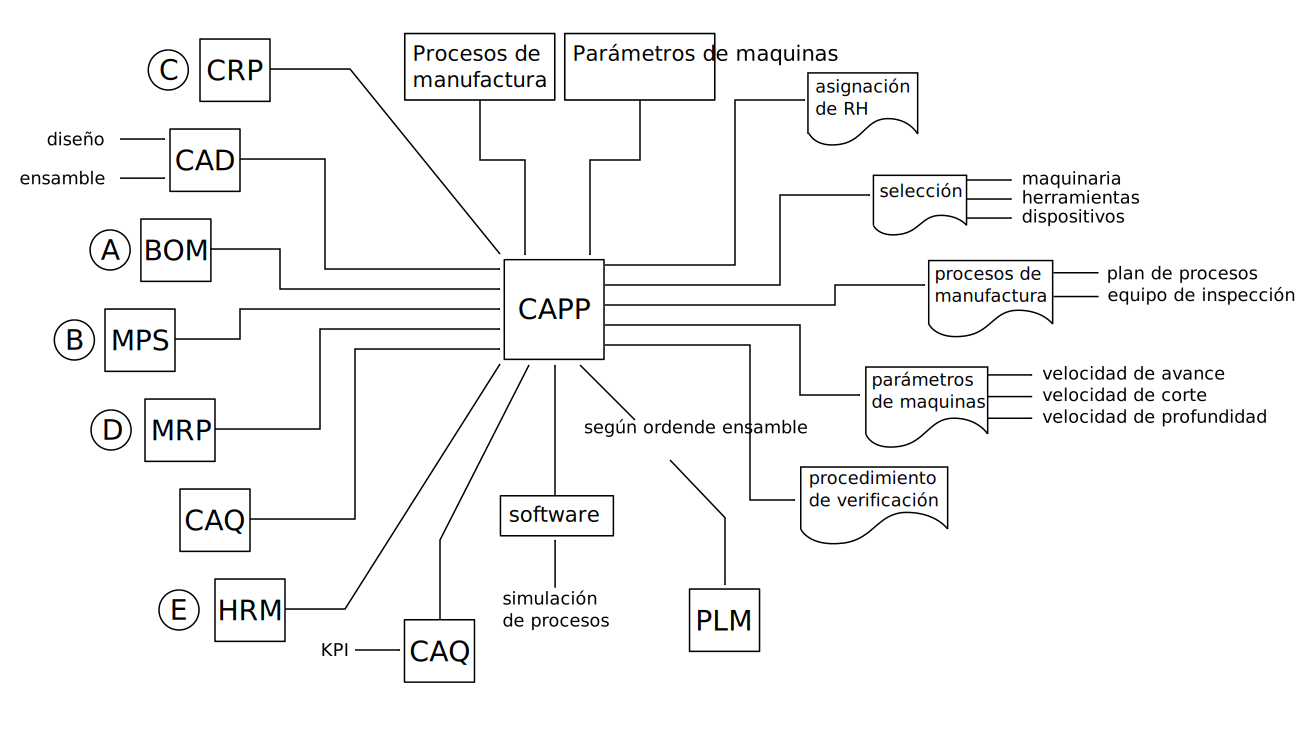
\includegraphics[scale=0.10]{Manufactura Integrada por Computadora Figuras/Figura08 CAPP.png}
        \caption{CAPP}
\end{figure}

Donde 
A: Matriz 
\begin{itemize}
    \item n: número de partes
    \item m: características 
\end{itemize}

B: Matriz
\begin{itemize}
    \item i: número de productos
    \item j: periodos
\end{itemize}

C: Matriz 
\begin{itemize}
    \item l: número de maquinas
    \item k: características de maquinas 
\end{itemize}

D: Matriz cubica 

E: Matriz 

En manufactura, el objetivo es producir componentes que cumplan con las especificaciones de diseño, ya que esta garantiza el aspecto funcional. El siguiente paso es ensamblar estos componentes en el producto final. 

La planificación de procesos actúa como puente entre el diseño y la fabricación de detalle. Por lo tanto, en general la planificación de procesos es una actividad de organización de producción que transforma un diseño de producto en un conjunto de instrucciones (secuencias, configuración de maquina, herramienta, etc.) para fabricar piezas mecanizadas de manera económica y competitiva. 

La información proporcionada en el diseño incluye especificación dimensional (forma geométrica y sus características) y especificación técnica (acabado superficial, tolerancia, etc.)